\clearpage
\section{Fase 6: Modelado y Ejecución}
En esta fase, el científico de datos diseña, crea o utiliza un modelo predictivo o descriptivo y lo alimenta con la versión del conjunto de datos o imágenes obtenidos en la fase de procesamiento y transformación. En esta fase, el científico debe seleccionar el tipo de aprendizaje (supervisado, no supervisado y por refuerzo) y la técnica determinada (regresión, clasificación, clustering, CNN, RNN, etc.) acorde a las preguntas planteadas en el \textit{BCQM}. Hay que mencionar que en esta fase el \textit{Data Analysis Team} debe definir junto al medico experto en oncología la tolerancia de error permitida en el modelo, esto dado a que la sensibilidad de los análisis puede variar dependiendo del tipo de cáncer de mama y la técnica de diagnostico. Es probable que el científico de datos pruebe múltiples algoritmos con sus respectivos parámetros para encontrar el mejor modelo para las variables oncológicas disponibles. Cabe resaltar, que es de vital importancia que los modelos propuestos no tengan problemas de sobre-ajuste o infra-ajuste ya que esto puede generar resultados erróneos o poco significativos. Adicionalmente, el científico de datos en cuestión junto al \textit{Data Analysis Team} deben definir la infraestructura a nivel de servidor necesaria para el entrenamiento y prueba del modelo según la cantidad de información a procesar, esto con el proposito de generar resultados acertados en el menor tiempo posible en pro de cumplir las tareas definidas en la fase de planeación de actividades y dar valor a los datos oncológicos una vez finalice el \textit{Release}.

\subsection{Agrupamiento(Clustering)}
Ahora bien, dado que las preguntas sobre el cáncer de mama planteadas en el BCQM se basan en datos de origen genómico y por ende tienen una representación simbólica con atributos cuantitativos y/o cualitativos en este caso de estudio se requiere un \textit{análisis diagnostico} para determinar las causas de las tendencias y las correlaciones entre las 41 variables oncológicas. Por lo tanto, se selecciono el  método de agrupamiento(\textit{Clustering}), ya que nos permite reunir los datos genómicos en clases o \textit{clusters} basados en los tipos de cáncer lobulillar invasivo(ILC) o ductal invasivo(IDC), de tal forma que es posible identificar que las variables de un determinado cluster tengan una similaridad alta o baja con respecto a los demás clusters.

Dado lo anterior, en la tabla \ref{Clustering_Models} se observan los algoritmos de agrupamiento que fueron ejecutados para posteriormente seleccionar el de mejor desempeño. Para ejecutarlos, se utilizó el lenguaje multi-paradigma \textit{Python} y la librería \textit{scikit-learn}, ya que permiten agilizar el entrenamiento de algoritmos de aprendizaje no supervisado.
\\\\
En este caso se realizó el análisis con base al agrupamiento de la totalidad de datos conformado por $818$ filas y $41$ columnas. Simultáneamente, para optimizar el modelo se utilizo el $95\%$ de los datos para el entrenamiento y el $5\%$ de datos restante para comprobar la precisión del agrupamiento y así poder de analizar los clusters generados. Cabe resaltar, que para la creación, entrenamiento y prueba del modelo se utilizo una maquina equipada con un procesador Intel Core i7-11370H de 11th generación con una frecuencia de 3.30 GHz-4.9 GHz , una tarjeta NVIDIA GeForce RTX 3050, un disco duro SSD Samsung con una velocidad de lectura de  7,000 MB/s y 48GB de memoria RAM. 

Para obtener el modelo de agrupamiento mas adecuado, se utilizaron la métricas de validación interna basadas en el índice de \textit{Davies-Bouldin} y el \textit{Coeficiente de silhouette}. Ademas, también se valido la cantidad de clusters generados para evaluar la eficacia en el agrupamiento de los datos. El resultado de este análisis puede ser observado en la figura \ref{TSNE}, la cual fue generada con el método T-SNE \footnote{T-SNE: T-distributed Stochastic Neighbor Embedding}, el cual genera una distribución de probabilidad que representa las similitudes entre vecinos en un espacio de gran dimensión y en un espacio de menor dimensión. 

Llegados a este punto, los modelos de agrupación \textit{Espectral(Spectral)} y \textit{Desplazamiento medio(Mean Shift)}  fueron los que presentaron un mayor valor en el coeficiente de Silhouette y un menor valor en el indice da Davies-Bouldin, respectivamente. Sin embargo al observar en la gráfica T-SNE del modelo de agrupación \textit{Espectral}, se pueden identificar 2 clusters, en donde el Cluster 0 abarca aproximadamente el 99\% del espacio con respecto al Cluster 1, por lo que en no existe una cohesión ni una separación clara de los datos. De la misma manera, el modelo de \textit{desplazamiento medio} presenta un comportamiento similar que aunque no se observa la gráfica T-SNE puede ser comprobado en la figura \ref{distance} que representa la distancia entre clusters con respecto a la posición inicial.

Finalmente, el modelo seleccionado para analizar el comportamiento de conjunto de datos del carcinoma invasivo de mama (TCGA, Cell 2015), fue el de \textit{agrupación BIRCH}, ya que no solo genero un coeficiente de silhouette  y un indice de Davies-Bouldin congruente sino también al validar la gráfica T-SNE se visualiza que los clusters presentan una metrica de cohesión y separación idónea.

\begin{table*} [!htb]
	\footnotesize
	\begin{threeparttable}
		\caption{Modelos Machine Learning para agrupamiento (Clustering).}
		\label{Clustering_Models}
		\begin{tabular}{p{1cm} p{6cm} p{2.5cm} p{2.5cm} p{1.5cm}} \toprule	
		\begin{center}Id\end{center}
		&\begin{center}Modelo Clustering\end{center}
		&\begin{center}Silhouette\end{center}
		&\begin{center}Davies-Bouldin\end{center}
		&\begin{center}Clusters\end{center}
		\\ \hline 1 & K-Means Clustering 	&	0,0826	&	2,5179	&	4
		\\ \hline 2 & Affinity Propagation	&	0,0518	&	2,2123	&	68
		\\ \hline 3 & Mean Shift Clustering 	&	0,2790	&	1,2792	&	7
		\\ \hline 4 & Spectral Clustering	&	0,7986	&	0,1419	&	2
		\\ \hline 5 & Agglomerative Clustering	&	0,1034	&	2,0468	&	4
		\\ \hline 6 & DB Spatial Clustering 	&	0,0000	&	0,0000	&	-1
		\\ \hline 7 & OPTICS Clustering	&	-0,2044	&	1,9565	&	10
		\\ \hline 8 & BIRCH Clustering	&	0,1286	&	1,8703	&	4
		\\ \hline 9 & K-Modes Clustering	&	0,0547	&	3,8189	&	3
		\\ \hline
		\end{tabular}
	\end{threeparttable}
\end{table*}

\begin{figure} 
	\setlength\tabcolsep{3pt}%%
	\centering
	\caption{Modelos Clustering aplicados al conjunto de datos del Carcinoma invasivo de mama (TCGA, Cell 2015).}
	\label{TSNE}
	\begin{tabular}{|c|c|}
		\hline
		\textbf{K-Means} &
		\textbf{Affinity Propagation} \\
		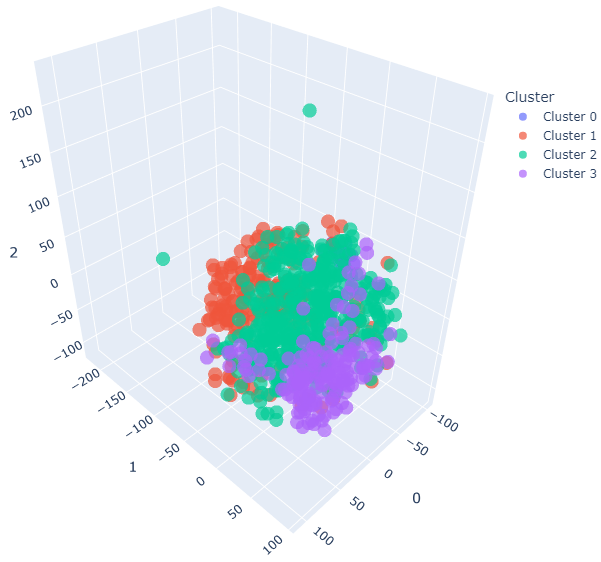
\includegraphics[width=0.5\textwidth]{NOTEBOOK/IMAGENES_CLUSTERING/1_TNSE_Kmeans} &
		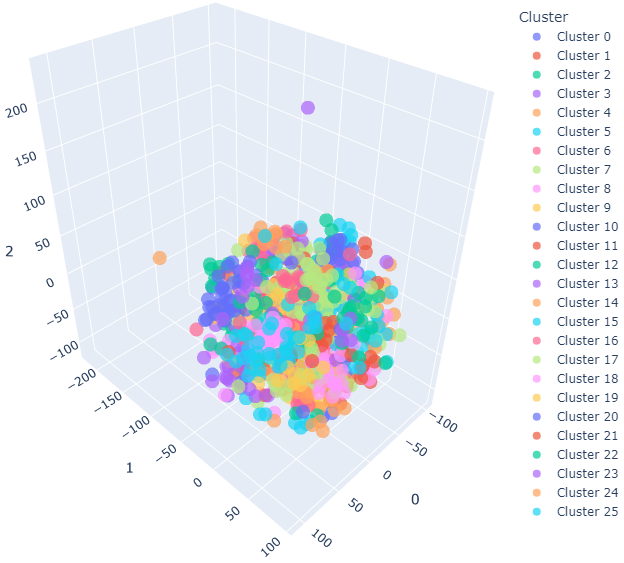
\includegraphics[width=0.5\textwidth]{NOTEBOOK/IMAGENES_CLUSTERING/2_TNSE_Affinity_Propagation} \\
		\hline
		
		\textbf{Mean Shift Clustering} &
		\textbf{Spectral Clustering} \\
		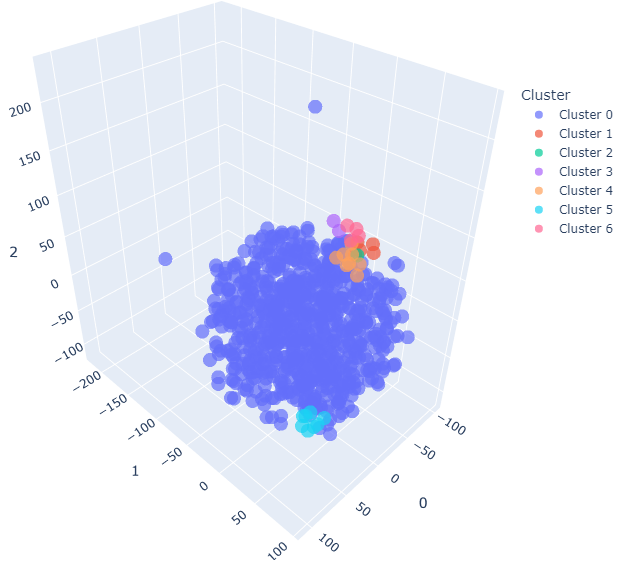
\includegraphics[width=0.5\textwidth]{NOTEBOOK/IMAGENES_CLUSTERING/3_TNSE_Mean_Shift_Clustering} &
		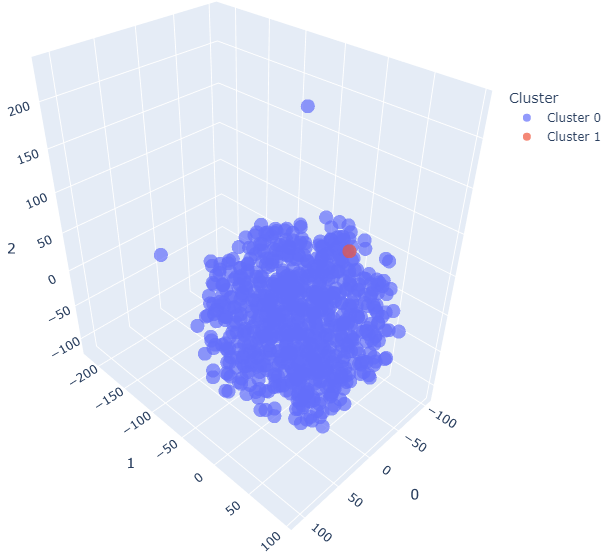
\includegraphics[width=0.5\textwidth]{NOTEBOOK/IMAGENES_CLUSTERING/4_TNSE_Spectral_ Clustering} 
		\\ \hline
	\end{tabular}
\end{figure}

\begin{figure} 
	\setlength\tabcolsep{3pt}%%
	\centering
	\begin{tabular}{|c|c|}
		\hline
		\textbf{Agglomerative Clustering} &
		\textbf{Density-Based Spatial Clustering} \\
		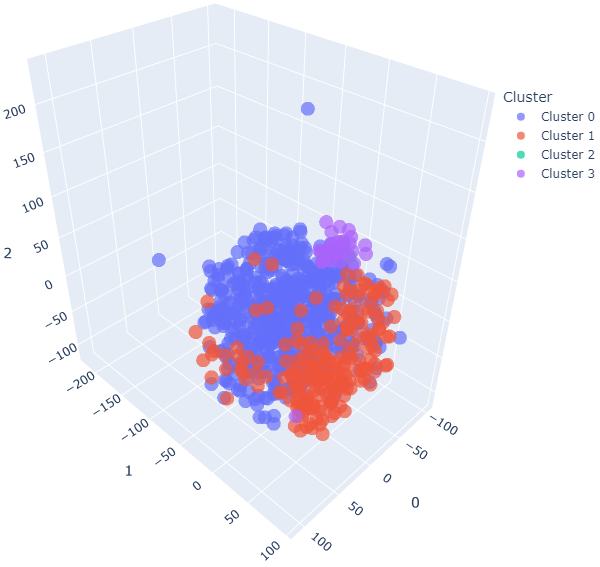
\includegraphics[width=0.5\textwidth]{NOTEBOOK/IMAGENES_CLUSTERING/5_TNSE_Agglomerative_Clustering} &
		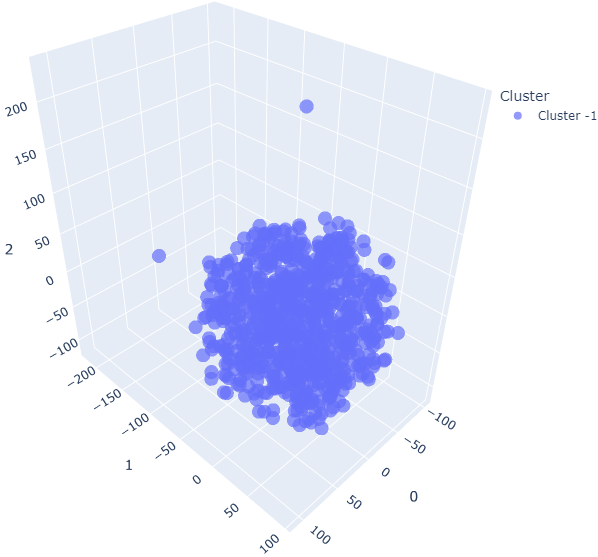
\includegraphics[width=0.5\textwidth]{NOTEBOOK/IMAGENES_CLUSTERING/6_TNSE_Density_Based_Spatial_Clustering} 
		\\ \hline
		\textbf{OPTICS Clustering} &
		\textbf{BIRCH Clustering} \\
		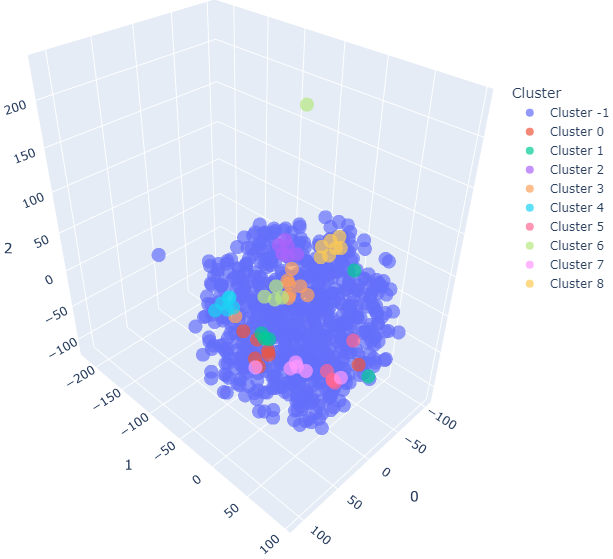
\includegraphics[width=0.5\textwidth]{NOTEBOOK/IMAGENES_CLUSTERING/7_TNSE_OPTICS_Clustering} &
		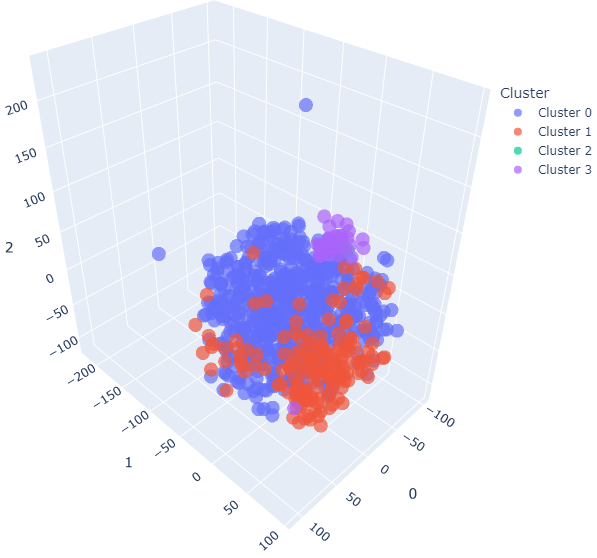
\includegraphics[width=0.5\textwidth]{NOTEBOOK/IMAGENES_CLUSTERING/8_TNSE_Birch_Clustering} 
		\\ \hline
	\end{tabular}
	\begin{tabular}{|c|}
	\hline
	\textbf{K-Modes Clustering} \\
	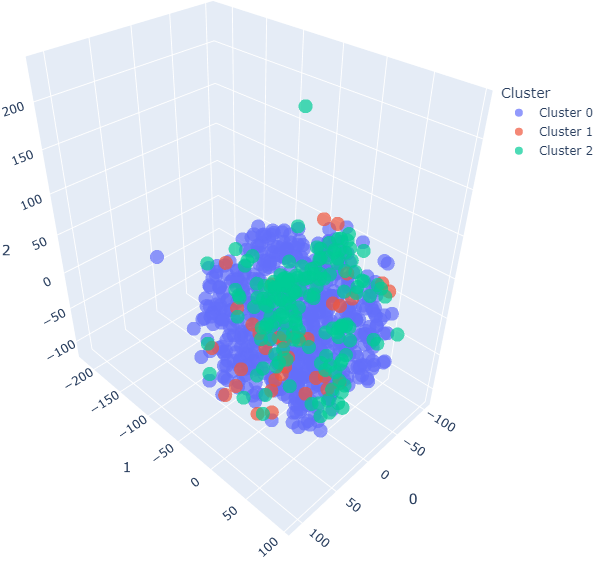
\includegraphics[width=0.5\textwidth]{NOTEBOOK/IMAGENES_CLUSTERING/9_TNSE_Kmodes}
	\\ \hline
	\end{tabular}
\end{figure}


\begin{figure} 
	\setlength\tabcolsep{3pt}%%
	\centering
	\caption{Mapas de distancia entre clusters de los modelos aplicados al conjunto de datos del carcinoma invasivo de mama (TCGA, Cell 2015).}
	\label{distance}
	\begin{tabular}{|c|c|}
		\hline
		\textbf{K-Means} &
		\textbf{Affinity Propagation} \\
		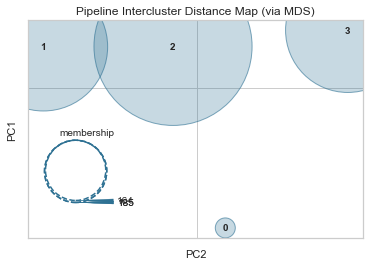
\includegraphics[width=0.5\textwidth]{NOTEBOOK/IMAGENES_CLUSTERING/1_MAP_Kmeans} &
		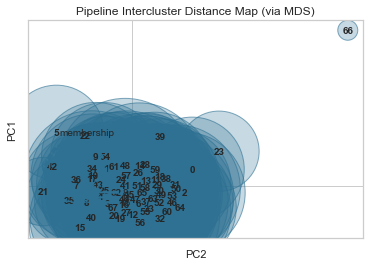
\includegraphics[width=0.5\textwidth]{NOTEBOOK/IMAGENES_CLUSTERING/2_MAP_Affinity_Propagation} 
		\\ \hline
	\end{tabular}
	\begin{tabular}{|c|}
		\hline
		\textbf{Mean Shift Clustering} \\
		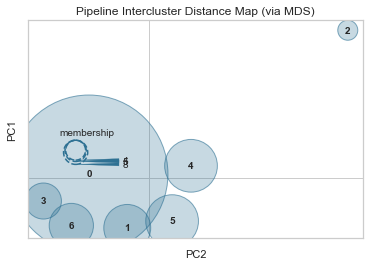
\includegraphics[width=0.5\textwidth]{NOTEBOOK/IMAGENES_CLUSTERING/3_MAP_Meanshift_Distance}
		\\ \hline
	\end{tabular}
\end{figure}


